%%%%%%%%%%%%%%%%%%%%%%%%%%%%%%%%%%%%%%%%%
% Jacobs Portrait Poster
% LaTeX Template
% Version 1.0 (31/08/2015)
% (Based on Version 1.0 (29/03/13) of the landscape template
%
% Created by:
% Computational Physics and Biophysics Group, Jacobs University
% https://teamwork.jacobs-university.de:8443/confluence/display/CoPandBiG/LaTeX+Poster
% 
% Further modified by:
% Nathaniel Johnston (nathaniel@njohnston.ca)
%
% Portrait version by:
% John Hammersley
%
% The landscape version of this template was downloaded from:
% http://www.LaTeXTemplates.com
%
% License:
% CC BY-NC-SA 3.0 (http://creativecommons.org/licenses/by-nc-sa/3.0/)
%
%%%%%%%%%%%%%%%%%%%%%%%%%%%%%%%%%%%%%%%%%

%----------------------------------------------------------------------------------------
%	PACKAGES AND OTHER DOCUMENT CONFIGURATIONS
%----------------------------------------------------------------------------------------

\documentclass[final]{beamer}

\usepackage[scale=1.24]{beamerposter} % Use the beamerposter package for laying out the poster

\usetheme{confposter} % Use the confposter theme supplied with this template

\setbeamercolor{block title}{fg=black,bg=white} % Colors of the block titles
\setbeamercolor{block body}{fg=black,bg=white} % Colors of the body of blocks
\setbeamercolor{block alerted title}{fg=white,bg=black!50} % Colors of the highlighted block titles
\setbeamercolor{block alerted body}{fg=black,bg=black!10} % Colors of the body of highlighted blocks
% Many more colors are available for use in beamerthemeconfposter.sty

%-----------------------------------------------------------
% Define the column widths and overall poster size
% To set effective sepwid, onecolwid and twocolwid values, first choose how many columns you want and how much separation you want between columns
% In this template, the separation width chosen is 0.024 of the paper width and a 4-column layout
% onecolwid should therefore be (1-(# of columns+1)*sepwid)/# of columns e.g. (1-(4+1)*0.024)/4 = 0.22
% Set twocolwid to be (2*onecolwid)+sepwid = 0.464
% Set threecolwid to be (3*onecolwid)+2*sepwid = 0.708

\newlength{\sepwid}
\newlength{\onecolwid}
\newlength{\twocolwid}
\newlength{\threecolwid}
\setlength{\paperwidth}{36in} % A0 width: 46.8in
\setlength{\paperheight}{48in} % A0 height: 33.1in
\setlength{\sepwid}{0.024\paperwidth} % Separation width (white space) between columns
\setlength{\onecolwid}{0.22\paperwidth} % Width of one column
\setlength{\twocolwid}{0.464\paperwidth} % Width of two columns
\setlength{\threecolwid}{0.708\paperwidth} % Width of three columns
\setlength{\topmargin}{-0.5in} % Reduce the top margin size
%-----------------------------------------------------------

\usepackage{graphicx}  % Required for including images

\usepackage{booktabs} % Top and bottom rules for tables

%----------------------------------------------------------------------------------------
%	TITLE SECTION 
%----------------------------------------------------------------------------------------

\title{Accelerating Artificial Neural Networks on Embedded FPGA with Hybrid Custom Floating-Point and Logarithmic Dot-Product Approximation} % Poster title

\author{Yarib Nevarez, Alberto Garcia-Ortiz} % Author(s)


\institute{Universit\"at Bremen, \href{mailto:nevarez@item.uni-bremen.de}{nevarez@item.uni-bremen.de},
\href{mailto:agarcia@item.uni-bremen.de}{agarcia@item.uni-bremen.de}} % Institution(s)

\newcommand\Fig[1]{\textbf{Fig.}~\ref{#1}}
\newcommand\fig[1]{\textbf{Fig.}~\ref{#1}}
\newcommand\Tab[1]{\textbf{Tab.}~\ref{#1}}
\newcommand\tab[1]{\textbf{Tab.}~\ref{#1}}
\newcommand\Equ[1]{\textbf{Eq.}~(\ref{#1})}
\newcommand\equ[1]{\textbf{Eq.}~(\ref{#1})}
\newcommand\Sect[1]{\textbf{Sec.}~\ref{#1}}
\newcommand\sect[1]{\textbf{Sec.}~\ref{#1}}
\newcommand\Refs[1]{\textbf{Ref.}~\cite{#1}}
\newcommand\refs[1]{\textbf{Ref.}~\cite{#1}}
\newcommand\Algo[1]{\textbf{Algorithm}~\ref{#1}}
\newcommand\algo[1]{\textbf{Algorithm}~\ref{#1}}

\begin{document}

\addtobeamertemplate{block end}{}{\vspace*{2ex}} % White space under blocks
\addtobeamertemplate{block alerted end}{}{\vspace*{2ex}} % White space under highlighted (alert) blocks

\setlength{\belowcaptionskip}{2ex} % White space under figures
\setlength\belowdisplayshortskip{2ex} % White space under equations

\begin{frame}[t] % The whole poster is enclosed in one beamer frame

\begin{columns}[t] % The whole poster consists of three major columns, the second of which is split into two columns twice - the [t] option aligns each column's content to the top

\begin{column}{\sepwid}\end{column} % Empty spacer column

\begin{column}{\onecolwid} % The first column

%----------------------------------------------------------------------------------------
%	ABSTRACT
%----------------------------------------------------------------------------------------

\begin{alertblock}{Abstract}

We accelerate artificial neural networks (ANN) optimizing the floating-point computation with vector dot-product approximation. The proposed method exploits the intrinsic error resilience of machine learning (ML) algorithms to reduce computational latency, memory footprint, and power dissipation while preserving inference accuracy. This method is integrated in a hardware/software co-design exploration framework. To demonstrate our approach, we address a hardware design exploration with convolutional neural networks (CNNs) and spiking neural networks (SNNs).
\end{alertblock}

%----------------------------------------------------------------------------------------
%	INTRODUCTION
%----------------------------------------------------------------------------------------

\begin{block}{Introduction}

%%%%%%% Contributions
We accelerate ANN with a dot-product hardware design based on approximate computing with hybrid custom floating-point and logarithmic number representation\cite{nevarez2021accelerating}. This hardware unit has a quality configurable scheme based on the bit truncation of the synaptic-weight vector. \fig{fig:dot_product_unit} illustrates the dot-product hardware module with standard floating-point (IEEE 754) arithmetic, and our approach with hybrid custom floating-point as well as logarithmic approximation. As a design parameter, the mantissa bit-width of the weight vector provides a tunable knob to trade-off between efficiency and quality of result (QoR)\cite{han2013approximate}. Since the lower-order bits have smaller significance than the higher-order bits, truncating them may have only a minor impact on QoR \cite{mittal2016survey}. Further on, we can remove completely the mantissa bits in order to use only the exponent of a floating-point representation. Therefore, the most efficient configuration becomes a logarithmic representation, which consequently leads to significant hardware-level optimizations using only adders and shifters for dot-product approximation. Moreover, since approximations and noise have qualitatively the same effect\cite{venkataramani2015approximate}, we propose noise tolerance plots as an intuitive visual measure to provide insights into the quality degradation of ANN under approximate processing effects.


\end{block}

\end{column} % End of the first column

\begin{column}{\sepwid}\end{column} % Empty spacer column

\begin{column}{\twocolwid} % Begin a column which is two columns wide (column 2)

\begin{columns}[t,totalwidth=\twocolwid] % Split up the two columns wide column

\begin{column}{\onecolwid}\vspace{-.6in} % The first column within column 2 (column 2.1)

%----------------------------------------------------------------------------------------
%	Design
%----------------------------------------------------------------------------------------

\begin{block}{Dot-Product Block-Level Design}

\begin{figure}
	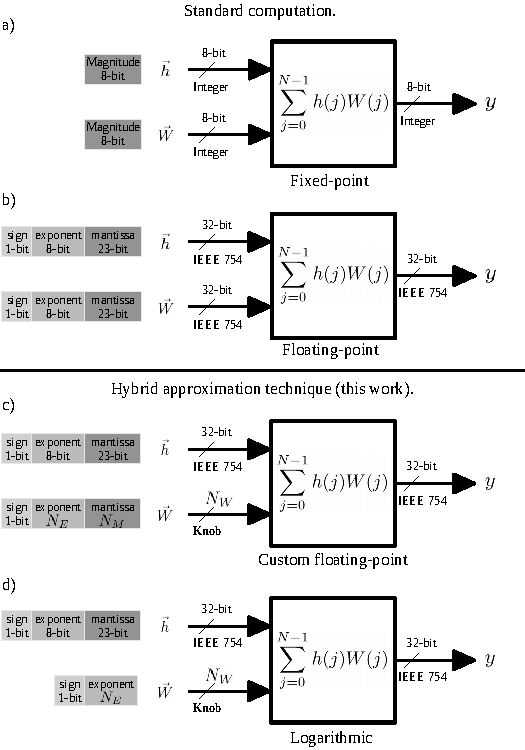
\includegraphics[width=\linewidth]{../figures/dot-product_unit.pdf}
	\caption{Hardware alternatives for vector dot-product.}
	\label{fig:dot_product_unit}
\end{figure}

\end{block}

\begin{block}{Tensor Processor}
		This section presents a tensor processor (TP) compatible with TensorFlow Lite to accelerate \emph{Conv2D} (\equ{eq:conv2D}) and \emph{DepthwiseConv2D} (\equ{eq:dconv2D}) operations on embedded FPGA. This TP instantiates the compute engines shown in \fig{fig:dot_product_unit}.
	\begin{figure}
		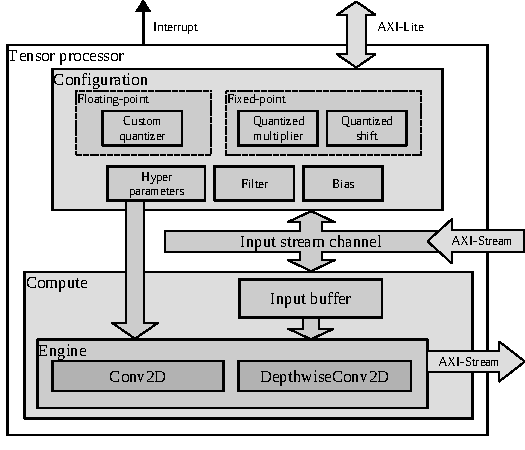
\includegraphics[width=\linewidth]{../figures/accelerator.pdf}
		\caption{Hardware architecture of the proposed tensor processor.}
		\label{fig:accelerator}
	\end{figure}
	
\end{block}
%----------------------------------------------------------------------------------------

\end{column} % End of column 2.1

\begin{column}{\onecolwid}\vspace{-.6in} % The second column within column 2 (column 2.2)

%----------------------------------------------------------------------------------------
%	SbS
%----------------------------------------------------------------------------------------

\begin{block}{Embedded System Architecture}
	\begin{figure}
		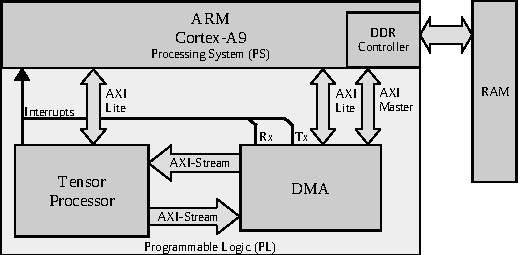
\includegraphics[width=\linewidth]{../figures/system_design.pdf}
		\caption{Base embedded hardware architecture.}
		\label{fig:conv_sys_design}
	\end{figure}
	
	\begin{figure}
		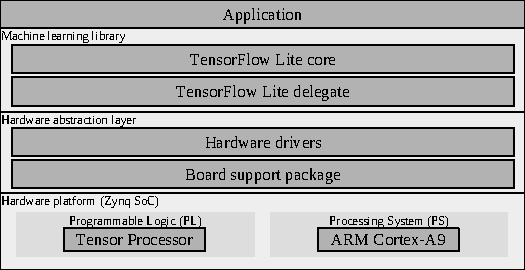
\includegraphics[width=\linewidth]{../figures/sw_stack.pdf}
		\caption{Base embedded software architecture.}
		\label{fig:embedded_sw}
	\end{figure}
\end{block}

\begin{block}{Experimental Results}
	A single TP achieves a peak acceleration of $45\times$ on \emph{Conv2D} tensor operation. The energy-delay product (EDP) of the different compute engines are compared in \tab{tab:energy}. The implemented custom floating-point formats and their classification accuracy are shown in \fig{fig:accuracy}.
	\begin{table}[!htp]\centering
		\caption{Energy consumption of a single TP at peak acceleration of 45X.}\label{tab:energy}
		\scriptsize
		\begin{tabular}{lrrrr}\toprule
			Engine &Power (W) &EDP (J) &Reduction \\\midrule
			CPU (ARM Cortex-A9)&1.404 &7,812.97 &1.00 \\
			TP (Fixed-point) &0.136 &16.67 &468.66 \\
			TP (Floating-point LogiCORE) &0.070 &39.85 &196.05 \\
			TP (Hybrid custom floating-point) &0.066 &8.19 &\textbf{954.43} \\
			TP (Hybrid logarithmic) &0.060 &7.40 &\textbf{1,055.92} \\
			\bottomrule
		\end{tabular}
	\end{table}
	
	\begin{figure}
		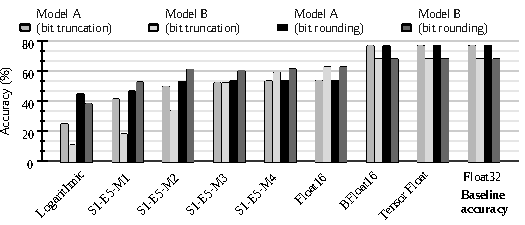
\includegraphics[width=\linewidth]{../figures/all_models_accuracy.pdf}
		\caption{Classification accuracy using hybrid custom floating-point approximation with various formats.}
		\label{fig:accuracy}
	\end{figure}
\end{block}

%----------------------------------------------------------------------------------------

\end{column} % End of column 2.2

\end{columns} % End of the split of column 2 - any content after this will now take up 2 columns width


\begin{alertblock}{Implemented operations}
	
\begin{eqnarray} \label{eq:conv2D}
Conv2D\left(W,X\right)_{i,j,o}=\sum_{k,l,m}^{K,L,M}W_{(o,k,l,m)} \cdot X_{(i+k,j+l,m)}+b_{o}
\end{eqnarray}


\begin{eqnarray} \label{eq:dconv2D}
DepthwiseConv2D\left(W,X\right)_{i,j,n}=\sum_{k,l}^{K,L}W_{(k,l,n)} \cdot X_{(i+k,j+l,n)}+b_{n}
\end{eqnarray}

\begin{eqnarray} \label{eq:sbs_update}
h_\mu^{new}(i) = \frac{1}{1+\epsilon} \left(h_\mu(i) + \epsilon \frac{h_\mu(i) W(s_t|i) }{\sum_j h_\mu(j) W(s_t|j)} \right) 
\end{eqnarray}

\end{alertblock} 

%----------------------------------------------------------------------------------------

\begin{columns}[t,totalwidth=\twocolwid] % Split up the two columns wide column again

\begin{column}{\onecolwid} % The first column within column 2 (column 2.1)

%----------------------------------------------------------------------------------------
%	MATHEMATICAL SECTION
%----------------------------------------------------------------------------------------


%----------------------------------------------------------------------------------------

\end{column} % End of column 2.1

\begin{column}{\onecolwid} % The second column within column 2 (column 2.2)

\end{column} % End of column 2.2

\end{columns} % End of the split of column 2

\end{column} % End of the second column

\begin{column}{\sepwid}\end{column} % Empty spacer column

\begin{column}{\onecolwid} % The third column

%----------------------------------------------------------------------------------------
%	CONCLUSION
%----------------------------------------------------------------------------------------

\begin{block}{Tolerance Plot}
	For quality monitoring, we propose tolerance plots as an intuitive
	visual measure to provide insights into the accuracy degradation of
	ANN under different approximate processing effects. This plot revels inherent error resilience, hence, the
	possibilities for approximate processing. \fig{fig:tolerance} shows the tolerance plot of a SbS network with hybrid logarithmic approximation \cite{nevarez2021accelerating}, this plot reveals elevated approximation resilience. The SbS dynamics is described in \equ{eq:sbs_update}.
	\begin{figure}
		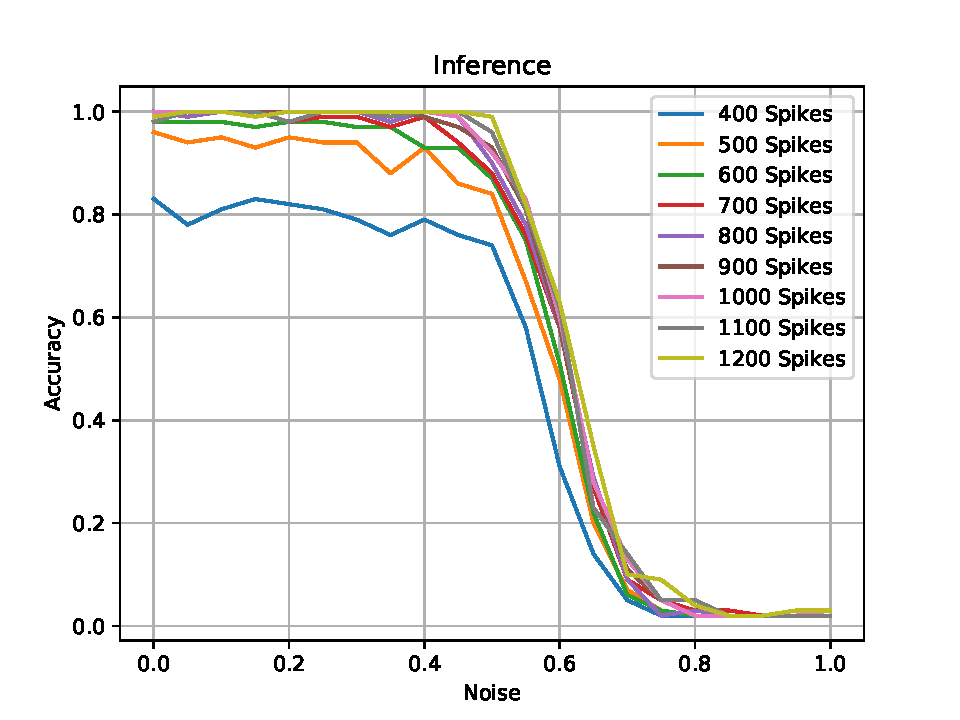
\includegraphics[width=\linewidth]{../figures/accuracy_vs_spike_log.pdf}
		\caption{Tolerance plot.}
		\label{fig:tolerance}
	\end{figure}
\end{block}

\begin{block}{Conclusions}
We present a hardware/software co-design framework to accelerate floating-point tensor computation in embedded FPGA with approximation techniques to reduce energy consumption and resource utilization.

\end{block}

%----------------------------------------------------------------------------------------
%	REFERENCES
%----------------------------------------------------------------------------------------

\begin{block}{References}

\nocite{*} % Insert publications even if they are not cited in the poster
\small{\bibliographystyle{unsrt}
\bibliography{sample}\vspace{0.75in}}

\end{block}

%----------------------------------------------------------------------------------------
%	ACKNOWLEDGEMENTS
%----------------------------------------------------------------------------------------

\setbeamercolor{block title}{fg=black,bg=white} % Change the block title color

\begin{block}{Acknowledgements}

\small{\rmfamily{This work is funded by \textit{CONACyT}.}} \\

\end{block}


\begin{center}
\begin{tabular}{ccc}

\includegraphics[width=0.4\linewidth]{../figures/logo_ub_2021.png} & \hfill & 
\includegraphics[width=0.4\linewidth]{../figures/logo_item_ids.png}
\end{tabular}
\end{center}

%----------------------------------------------------------------------------------------

\end{column} % End of the third column

\end{columns} % End of all the columns in the poster

\end{frame} % End of the enclosing frame

\end{document}
